% !TeX root = ../main.tex

\chapter{相关工作}

卷积是在深度学习和图像处理中最为常用的一种操作,直观而言,卷积神经网络中的卷积操作可以理解为
将卷积核在图像上滑窗,并这个位置计算卷积核与对应的图像输入位置像素的点积并输出到对应的位置。

卷积核大小为$k_1xk_2$的卷积操作作用于大小为$MxN$的矩阵的直接卷积算法具有$O(MNk_1k_2)$
的计算复杂度,而对于存储的复杂度则为$O(MN)$。因此,从理论上讲,像GEMM(矩阵乘法,也称为
Dense Layer, 线性层(Linear layer)或仿射层(Affine Layer))一样,,卷积是受计算限制
(compute bounded)的操作不是为内存限制(memory bouned)的操作。
同时,对于多通道的图像输入,内存复杂度变为$O(MNC)$,计算复杂度变为$O(MNCk_1k_2)$。


\section{卷积实现方法概述}

\subsection{直接卷积方法}

由于通用矩阵乘法(GEMM)和卷积都是受到计算资源限制的操作(computation bounded operation),
用于实现高效矩阵乘法的很多方法可以借鉴被用于提高卷积操作的效率。Cache blocking 和 Register
blocking 是常用的用于实现高效矩阵乘法的两种策略,值得注意的是,这两种策略并不改变矩阵乘法的
算法复杂度$O(n^3)$,而是从硬件角度考虑,充分利用到硬件的计算资源,对矩阵乘法实现硬件友好(hardware
friendly)的重新调度。 工作
\cite{Georganas2018AnatomyOH} 和
\cite{Zhang2018HighPZ}
中的直接卷积方法实现均借鉴了
这一对于矩阵乘法的优化策略,不改变卷积计算本身的复杂度,而是对于直接卷积计算考虑更加硬件
友好的实现:

对于卷积操作输入的四个维度,这里记minibatch 的大小为N,输入的feature map的数目为 C,空间
尺度为 HxW, 而与之对应的输出的feature map数目,或者说输出的通道数为K,输出特征的空间尺度为
PxQ,以及卷积操作由四维张量所表示的权重,各个维度的尺度分别为,输入和输出的特征通道数C, K 
卷积核的空间维度 R和S。

于是直接卷积算法的处理过程中,如Algorithm \ref{algo:direct-conv}所示,具有6重循环,其中输入的特征
为I,卷积的权重为W,而输出的特征为 O 

\begin{algorithm}
  \caption{直接卷积实现}
  \KwIn{Input image $I$, Kernel $W$}
  \KwOut{ Ouptut feature $O$}
  \For{ $k$ \gets 1 \KwTo $K$}{
    \For{ $c$ \gets 1 \KwTo $C$}{
      \For{ $p$ \gets 1 \KwTo $P$}{
        \For{ $q$ \gets 1 \KwTo $Q$}{
          \For{ $r$ \gets 1 \KwTo $R$}{
            \For{ $s$ \gets 1 \KwTo $S$}{
                $O_{n,k,p,q} += I_{n,c,p+r,q+s} \times W_{k,c,r,s}$
              }
            }
          }
        }
      }
    }
  \label{algo:direct-conv}
\end{algorithm}

而考虑到现代主流硬件普遍支持向量化处理(vectorization)的并行计算,在对应的架构下,处理器
有矢量寄存器(vector register)实现数据的并行化处理。而这一并行处理的
过程同处理器架构和数据类型相关,比如对于x86架构的AVX512 矢量计算,如果输入为32位浮点数
那么计算过程中可以支持16个32位浮点数的并行计算。而为了充分利用矢量寄存器的并行处理能力,需要
将计算中最内层,迭代最为频繁的这一维度的数据,分块打包成大小同矢量寄存器所能容纳数据的最大值相等
的子块。比如上述的AVX 512 矢量计算中,需要将计算最内层的数据分为多个16个32位浮点数组成的小块。
除此之外,在寄存器层面,可以
使用 register blocking 技术实现寄存器中的数据复用,并减小L1 缓存中的数据传输压力,以期
减小操作延时。\cite{Georganas2018AnatomyOH} 中将 register blocking 应用在输出特征的
空间维度层面上,因此在空间维度的迭代过程中,其中的每个点的值均可以独立计算。
在综合了寄存器角度的优化策略之后,即矢量化(vectorizatoin)和 register blocking,
\cite{Georganas2018AnatomyOH} 对于直接卷积算法提出了如Algorithm\ref{algo:opt_direct_conv}
所示的优化,这里 $C_{o,b}$ 表示经过Blocking 方法实现的输出通道量的分块,算法中针对$W$ 的表示类似。

\begin{algorithm}
  \caption{优化直接卷积算法}
  \KwIn{Input image $I$, Kernel $W$, stride $s$}
  \KwOut{ Ouptut feature $O$}
  \For{ $\tilde{j} \gets 1$ \KwTo $C_o / C_{o,b}$}{
    \For{ $\tilde{i} \gets 1$ \KwTo $C_i / C_{i,b}$}{
      \For{ $l \gets 1$ \KwTo $H_o$}{
        \For{ $\tilde{k} \gets 1$ \KwTo $W_o / W_{o,b}$}{
          \For{ $n \gets 1$ \KwTo $H_f$}{
            \For{ $m \gets 1$ \KwTo $W_f$}{
              \For{ $ii \gets 1$ \KwTo $C_{i, b}$}{
                \For{ $kk \gets 1$ \KwTo $W_{o,b}$}{
                  \For{ $jj \gets 1$ \KwTo $C_{o, b}$}{
                    $O_{\tilde{j}C_{o,b}+jj, \tilde{k}W_{o,b}+kk,l} +=
                    I_{\tilde{i}C_{i,b}+ii,s\tilde{k}W_{o,b}+kk+m,ls+n} \times
                    W_{\tilde{i}C_{i,b}+ii,\tilde{j}\times C_{a,b}+jj,m,n}$
                  }
                }
              }
            }
          }
        }
      }
    }
  }
  \label{algo:opt_direct_conv}
\end{algorithm}

直接卷积乘法无需考虑额外的变换,也没有额外的储存需求,因而在存储角度考虑实际上是相当高效的,
而且直接卷积算法也不对卷积本身的设定有任何的预设,可以直接应用于各种类型的卷积操作。而另外一方面,
直接卷积算法的缺陷也同样是显而易见的,这一实现实际上对于缓存相当不友好。对于相当常用的 3x3 卷积
而言,如果输入的数据类型使用32位表示,在计算第一行中的输入的3个值的过程中会加载与其位于同一缓存
行中的16个值,而在下一步的计算中,CPU需要处理下一行中的3 个数值,同时又会将这些值位于同一缓存行
中的值加载到缓存中,而直到第三行的数据操作完毕之后,由于缓存的容量一般很小,第一行的数据已经从
缓存中抹去了,而这时的计算却正好需要这些数据。 这些存储访问相关的问题都会限制计算密度的最大化和计算资源的最有效利用。

\subsection{基于GEMM 的卷积实现}

\subsubsection{Im2col (Image to Columns)}

Im2col(Image Block to Column)是当前最流行的CPU卷积方案。这一卷积实现方法自Caffe\cite{Jia2014CaffeCA}起,便在
卷积神经网络计算的实现中有着相当广泛的支持,而也正是caffe使得基于GEMM的卷积实现方法得以流行。
这一方法最早建于\cite{Chellapilla2006HighPC} 它依赖于经过数十年优化的矩阵乘法(GEMM),以充分利用CPU缓存。
这样的优点是计算速度更快,但会占用更多的内存。 使用im2col运算将输入图像转换为矩阵,
然后将该矩阵与变换后的卷积核相乘。 最后,再使用col2im操作将这个相乘后的矩阵重新转换为图像。

从微观角度来看,卷积操作基本上就是卷积核参数同移动窗口所选择的同卷积核尺度相同的局部区域
之间的点积(dot product)。Im2col 的基本想法就在于将所有可能的窗口在内存中展开,然后
使用矩阵乘法实现点积,毕竟点积和矩阵乘法的基本流程都是对应位置乘积的和(sum of element-wise
product)。从而可以用更大的内存消耗为代价而换取实现的简化和计算加速,

简而言之,im2col技术,每个窗口截取,将其展平,然后将它们堆叠为矩阵中的列。 再将内核展平
为行向量并在两者之间进行矩阵乘法,则在输出reshape后可以获得完全相同的结果。
\begin{figure}
	\centering
	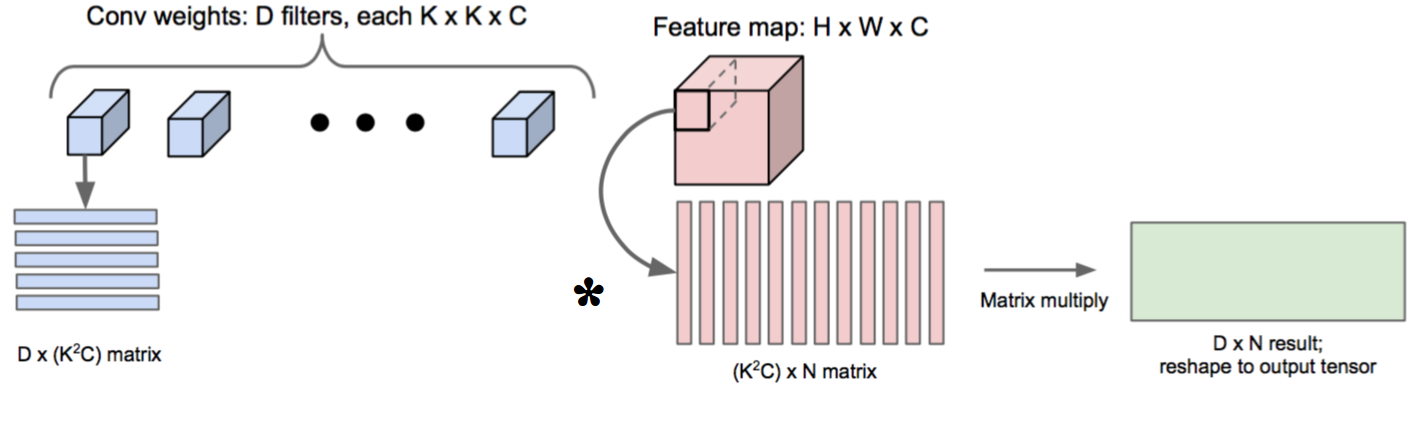
\includegraphics[width=0.8\columnwidth]{Im2col.png}
	\caption{Im2Col 方法}
	\label{fig:im2col}
\end{figure}

% Im2col 的简单伪代码表示如\ref{algo:im2col} 所示,
% 
% \begin{minted}{python}
% \caption{im2col实现}
%   def im2col(x, kernel_shape):
%     # x is input activation
%     rows = []
% 
%     # Assuming Padding = 0, stride = 1
%     for row in range(x.shape[0] - 1):
%         for col in range(x.shape[1] - 1):
%             window = 
% 	    x[row: row + kernel_shape, col: col + kernel_shape]
%             rows.append(window.flatten())
%     return rows.transpose()
% \label={algo:im2col}
% \end{minted}

在im2col 方法中内存复制的复杂度为$O(MNC)$, 而卷积的复杂度为 $O(MNCk_1k_2)$,因此,在
大多情形下,内存复制所需要的时间开销同卷积本身相比仍然较低的,并且在卷积核尺度较小的场景下
Im2col方法的内存复杂度相对而言也是可接受的,从而总体上im2col 可以实现
对于卷积操作的加速。


\subsubsection{Memory Efficient Convolution}

MEC 方法\cite{Cho2017MECMC}作为对于im2col 的一种改进和扩展,旨在改善im2col 方法中对于内存的额外需求。
Im2col 实际是一种矩阵的降维手段(lowering scheme),将输入的3D 张量通过im2col可以转换
为 2D 矩阵并且可以直接使用BLAS 实现来完成矩阵乘法。Im2col 的方法变换之后的矩阵中存在着
相当多的数据冗余,这也表示这种方法可以通过去除这其中的数据冗余实现对于im2col 方法中过多
的memory overhead。Im2col 方法会将 $ W_i \times H_i \times C_i $ 的三维张量转换为 
$(H_f \times W_f \times C_i) \times (H_o \times W_o) $ 的二维矩阵,可见这一过程中,
额外需要的内存会随着问题规模存在着平方级别的增长趋势。

Im2col 方法中将输入的矩阵中的一个子块做降维,同Im2col方法不同的是, MEC 方法在实现的
过程中会一次将多列值降维,并且通过额外的矩阵乘法调用减少冗余的内存占用。

\begin{figure}
  \centering
  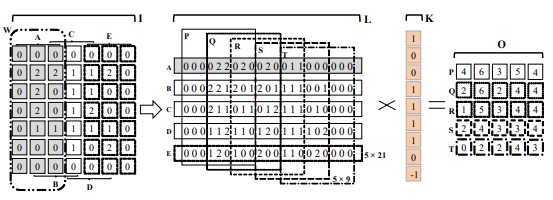
\includegraphics[width=0.8\columnwidth]{mec.png}
  \caption{MEC 卷积方法}
  \label{fig:mec}
\end{figure}

如图\ref{fig:mec} 中所示,对于一个 7x7 的输入,和3x3 的卷积核,这里需要实现降维的对象是
输入矩阵中的3列数据,记输入为 I,则这里需要将 $ I[0:7, 0:3] $ 这一区域中的数据平摊为一维,
即图中的第二步所示,依次按照滑窗实现输入的按照列的降维,在stride 为1 的情形下,这里在第二步
得到了降维后的 5 个一维向量,构成一个 5x 21的矩阵,而在实现矩阵乘法的过程中,则又需要
对于这个 5x21 的矩阵做划分为5x9 的子矩阵,在划分的过程中每向右移动三个单位(横向stride 乘
卷积核宽度)取一个子矩阵。每一个子矩阵和平摊(flatten)为一维向量的卷积核之间的乘积构成输出
的一行。 尽管这一过程中需要更多的矩阵乘法调用,但实际的乘法/加法操作则同im2col方法一致。
在计算复杂度上没有变化。


MEC 方法可以有效的减少im2col方法中在垂直方向上的数据冗余,在上图所示的计算过程中已经达到了
相对于im2col 方法54\% 的存储开销减少。这种方法甚至可以达到相对于im2col方法3.2 倍的存储资
源节省。

\subsection{快速卷积方法实现}

前面所提到的卷积算法,其优化的出发点都在于将卷积实现本身以高性能计算的角度解决问题(直接卷积方法),
或者说将卷积转换为研究相对充分的高性能计算问题(基于GEMM的方法),而对于卷积操作本身的复杂度
和运算量均没有实质性的降低。而卷积这一源自于信号处理的概念,则实际上在信号处理方法中已经有着
相当长远的研究,并且存在着很多可以实现卷积计算复杂性简化的方法。这些方法的主要目的在于减少卷积实现中的乘法
操作。因此这一类方法被称为快速卷积方法。

\subsubsection{FFT 卷积}
从信号处理中的角度而言,频域中的乘法对应于时域中的卷积。 使用DFT将输入信号转换到频域,再乘以滤波器的频率响应,然后使用Inverse DFT将输入信号转换回时域。
从傅立叶时代开始这种基本技术就广为人知。 但是,因为计算DFT所需的时间比直接计算卷积所需的时间长,所以使用傅里叶变换实现卷积的方法并没有受到足够的重视。
随着1965年快速傅立叶变换(FFT)的发展,这种情况发生了变化。 通过使用FFT算法计算DFT,与直接对时域信号进行卷积相比,通过频域进行卷积可以更快。而卷积的运算量
则获得了有效的缩减。一般而言,2维场景下,直接卷积的计算复杂度为 $O(n^4)$, 而FFT 卷积则可以将计算复杂度降低到 $O(n^2 \log_{2}n)$。而具体的在FFT 卷积
中的每一个步骤所需的计算复杂度同直接卷积方法的对比可以参考工作\cite{Mathieu2013FastTO}。

基于FFT的卷积方法\cite{Zlateski2018FFTCA} \cite{Mathieu2013FastTO}可以表示为

\begin{align}
  f * g = F^{-1}(F(f)  \cdot F(g))
\end{align}
其中的$F$ 与 $F^{-1}$ 表示傅里叶变换和逆傅里叶变换,在离散场景下,$f$ 和 $g$ 需要具有相同数目的元素,这一点可以通过向两者中较短的那一方实现 zero padding实现。
DFT卷积的结果是一个循环卷积(circular convolution/ cyclic convolution),而从中获得有效的卷积结果仍然需要从循环卷积的结果中抽取其中的最后 $|f| - |g| + 1 $
个元素。

在FFT 卷积方法中,卷积的输入和权重在经过离散傅里叶变换之后被变换为复数表示,而此后则需要执行二者之间的复数矩阵乘法。而在这一过程中,又具有着以下两种
特性能够进一步降低乘法操作的数目。

\begin{itemize}
  \item 实数值傅里叶变换的 Hermitian 对称性;
  \item 快速复数乘法计算;
\end{itemize}

实数域中的信号的 FFT 变换是具有 Hermitian 对称性(Hermitian symmetry)的, 即实数矩阵在傅里叶变换之后的矩阵同其共轭转置矩阵(conjugate transpose)是相等的,
这使得在 FFT 卷积方法中的矩阵乘法部分的实际有效乘法量可以进一步减半。一个尺寸为 $m x m$ 的实数值矩阵的离散傅里叶变换由于 Hermitian 对称性可以用 $ m x (floor(\frac{1}{2} + 1)) $ 
个复数来表示。同时又由于 $ U^H V^H = ( UV )^H $,矩阵乘法结果中的一半元素的值(上/下三角)可以通过取已计算值的共轭获得。

\paragraph{复数乘法计算}
复数计算在信号处理中有着广泛的应用,然而不幸的是,很多现代硬件在底层的指令上则缺少直接计算复数计算的支持,这使得复数计算的实现不得不面临着额外的挑战和付出。
而针对于ARM平台,尽管在ARMv8.2指令集(ISA) 之后添加了 FCADD (Floating-point Complex Add), FCMLA (Floating-point Complex Multiply Accumulate) 操作,
然而实现这一指令集的芯片微架构(microarchitecture)并不占据主流,主要集中在高端智能收集芯片上,比如苹果应用于iPhone X上的A11芯片及其之后的应用于iPhone XS系列的
A12芯片以及iPhone 11 的 A13芯片,在很多的嵌入式设备场景下的low profile的计算资源场景下,指令级别的复数操作支持仍然是缺失的。

一般的复数乘法中,一对复数相乘需要四次复数乘法,即

\begin{align}
\label{eq:complex_mul}
(u_r + i u_i)(v_r + i v_i) = u_r v_r - u_i v_i + i ( u_i v_r + u_r v_i )
\end{align}

而对于\ref{eq:complex_mul} 稍加变换既可以得到复数乘法的快速算法,该方法只需要三个实数乘法。

\begin{align}
\label{eq:complex_mul_fast}
  (u_r + i u_i) (v_r + i v_i) &= [ u_r v_r - u_i v_i, i(u_r v_i + u_i v_r)]\\
                               &= [ u_a - u_c,i( u_a + u_b) ]
\end{align}

where 
\begin{align}
u_a = v_r ( u_r + u_i )\\
u_b = u_r ( v_i - v_r )\\
u_c = u_i ( v_r + v_i )
\end{align}

这一方法,通过使用更多的加法实现在复数乘法计算过中乘法的减少 。

\paragraph{快速复数乘法在傅里叶卷积中的应用}

在执行图像块的变换后,产生一个复数张量 $U = U_r + i U_i$ ,可以计算实值张量 $U_r + U_i$ 并将其与Ur和Ui一起存储。 类似地, 卷积核权重在离散傅里叶变换之后得到一个
复数张量 $V = V_r + i V_i $, 张量 $V_i - V_r$ 和 $V_r + V_i$ 可以在内核变换期间计算, 并与 $V_r$ 一起存储(不必存储$V_i$ )。这里每个变换前的实数域的输入
对应于变换后的三个实数值,而不是直观理解上的每个变换后的值对应两个用来表示复数实部和虚部的两个实数。 然后,可以用三个独立的实值张量的元素间乘积替换复数张量的
元素间乘积. 而由此计算得到的三个 实数张量则可以在计算逆变换的过程中被隐式的转换为单个实数张量。总体来讲,快速复数乘法的实现,可以使得原本的复数域中的一个矩阵间
乘法转换为3个实数域中的矩阵乘法, 同直接计算复数乘法相比,可以将乘法的操作数减少 25\%.

FFT 卷积在执行计算的过程中需要将权重填充到和输入同等大小,这回导致额外并且不必要的内存负担,特别是在
卷积核本身毕竟小的状态下。信号处理中对于这一问题也有着比较成熟的解决方案,即 overlap add 和 overlap save
方法。切换到深度学习的场景下,可以实现对于输入的图像的切分,在每个小块上执行FFT 卷积,再将得到的结果
通过类似overlap add / overlap save的方法拼凑为整个图像输入的结果。 但是,这样的方法还需要将内核权重
填充到合适的大小(通常为2的幂)以达到最优性能。 即使将内核权重填充到架构寄存器大小的较小倍数(例如8或16)
,也会导致内存需求增加7到28倍。 此外可以通过动态执行FFT, 将FFT作为卷积层计算的一部分来最小化这种额外填充
卷积核权重并将其转换到频域的overhead。 但是,这会产生大量的性能开销,使得资源受限的嵌入式设备雪上加霜。


\subsubsection{Winograd 卷积}

Winograd minimal filtering算法是在信号处理中常用的一类快速算法,并且在信号处理领域已经有了相当时间的应用和研究。而
近年来\cite{Lavin2015FastAF} 才将这一方法引入卷积网络的计算中。下面将从卷积网络计算的角度,考虑这一算法在
卷积计算中的具体应用场景,简要解释介绍Winograd 算法对于卷积计算过程的优化。

从1D 的卷积过程来考虑,对于卷积核大小为3 的情形,对于连续两次的卷积过程,如图\ref{fig:conv_slide}
所示,输出 $r_0$ 由输入$k_0, k_1, k_2$ 同卷积核参数做元素间乘法相加得到,同样的,输出中的 $r_1$ 
则由输入$k_1, k_2, k_3$ 计算得出,这一过程中输出两个值需要有4个输入,将这一过程用矩阵乘法来做表示

\begin{figure}
\centering
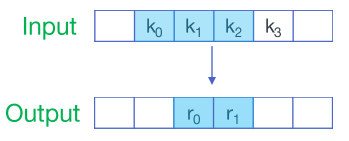
\includegraphics[width=0.5\columnwidth]{conv_sliding.png}
\caption{1D 卷积}
\label{fig:conv_slide}
\end{figure}


\begin{align}
  \begin{pmatrix}
    k_0 & k_1 & k_2 \\
    k_1 & k_2 & k_3 
  \end{pmatrix}
  \begin{pmatrix}
    w_0\\
    w_1\\
    w_2
  \end{pmatrix}
  =
  \begin{pmatrix}
    r_0 \\
    r_1
  \end{pmatrix}
\end{align}

直接做矩阵乘法,这一过程需要 6 次乘法和 4次加法:

\begin{align}
  r_0 = k_0 w_0 + k_1 w_1 + k_2 w_2 \\
  r_1 = k_1 w_0 + k_2 w_1 + k_3 w_2 
\end{align}

而如果对上述的乘法计算过程做如下的变换:

\begin{align}
\label{eq:winograd_mul}
  \begin{pmatrix}
    k_0 & k_1 & k_2 \\
    k_1 & k_2 & k_3 
  \end{pmatrix}
  \begin{pmatrix}
    w_0\\
    w_1\\
    w_2
  \end{pmatrix}
  =
  \begin{pmatrix}
    m_0 + m_1 + m_2 \\
    m_1 - m_2 - m_3
  \end{pmatrix}
\end{align}

其中,

\begin{align}
  m_0 = (k_0 - k_2) w_0\\
  m_1 = (k_1 + k_2) \frac{w_0 + w_1 + w_2}{2}\\
  m_0 = (k_0 - k_2) w_0\\
  m_2 = (k_2 - k_1) \frac{w_0 - w_1 + w_2}{2}
\end{align}

由于在卷积的过程中,卷积核权重的值都是确定的,所以其中 $m_1, m_2$中同 $w$ 相关
的这一部分均可以在计算矩阵乘法(卷积操作)之前预先计算。从而这一过程可以将
乘法的数目减少到4次,而上述的这一过程即为 $F(2, 3)$ 卷积在1D 场景下的实现,
而二维的场景,只需要将1D 的场景做进一步的嵌入即可实现。

具体而言,对于如图所示的 $F(2x2, 3x3)$ 的场景
\begin{figure}
\centering
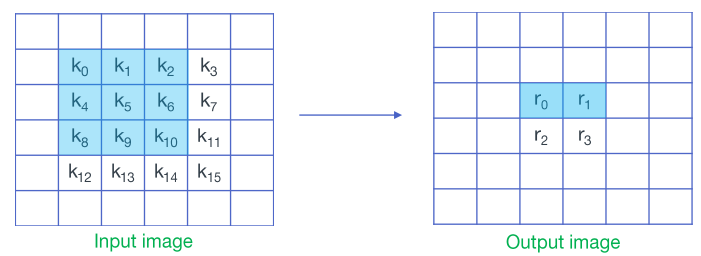
\includegraphics[width=0.8\columnwidth]{conv2x2_3x3.png}
\caption{F(2x2, 3x3) 卷积}
\label{fig:conv2x2_3x3}
\end{figure}

用矩阵乘法的形式表示这一卷积过程

\[
\label{eq:f2x3}
  \begin{pmatrix}
    k_0 & k_1 & k_2 & k_3 & k_4 & k_5 & k_6 & k_7 & k_8 & k_9 & k_10 \\
    k_1 & k_2 & k_3 & k_4 & k_5 & k_6 & k_7 & k_8 & k_9 & k_10 & k_11 \\
    k_4 & k_5 & k_6 & k_7 & k_8 & k_9 & k_10 & k_11  & k_12 & k_13 & k_14 \\
    k_5 & k_6 & k_7 & k_8 & k_9 & k_10 & k_11 & k_12 & k_13 & k_14 & k_15
  \end{pmatrix}
  \begin{pmatrix}
    w_0 \\
    w_1 \\
    w_2 \\
    w_3 \\
    w_4 \\
    w_5 \\
    w_6 \\
    w_7 \\
    w_8
  \end{pmatrix}
  = 
  \begin{pmatrix}
    r_0 \\
    r_1 \\
    r_2 \\
    r_3
  \end{pmatrix}
\]

类比于 1D 场景下的处理方法,这里可以得到相似的处理形式,不同点在于,1D 场景下简化
的乘法\ref{eq:winograd_mul}中表示的值均为Scalar,而2D场景下对应的值为一个子矩阵,
可见在2D 场景下,乘法操作的数目可以由直接矩阵乘法计算的36次,减少到16次,从而以
乘法计算的复杂度来考虑,可以达到 2.25 倍的复杂度降低。

\subsubsection{FFT 卷积实现同Winograd 卷积的对比}

离散傅里叶变换方法的有效卷积可以视作 Winograd 卷积 \ref{eq:winograd1d} 的一种特殊情形,其中的矩阵$A^T$, $B^T$ 和 $G$ 均处于复数域,并且由多项式点
( polynomial point)为单位根的范德蒙矩阵(Vandermonde matrices)推导出。

Winograd 与 FFT 卷积中主要能够降低计算成本的一点在于,权重的变换可以预先计算,而卷积输入的变换则可以多次复用,而计算本身中比重最大的部分仍然是矩阵乘法,而矩阵乘法的规模正好通过变换过程得以降低。


\section{神经网络量化研究}

减小计算资源的需求并提高功耗利用是在边缘设备上实现智能应用的一大挑战。量化方法
便是解决这一挑战的一条可行的途径。量化过程做一个简单的比喻,可以理解为是图片的
编码,现实世界中的图像视觉信号是连续的模拟信号,量化过程便是使用有限的编码位数,
用离散的整数值逼近重建实际的连续值。

在机器学习应用中,神经网络由激活节点,节点之间的连接以及与每个连接关联的权重参数组成。
这些权重参数和激活节点计算可以量化。在硬件上运行神经网络往往存在着数百万的乘法
和加法运算。 具有量化参数的低位数学运算与对神经网络的中间计算进行量化相结合,
可带来较大的计算增益和更高的性能。

\subsection{网络模型量化方法}
量化网络模型在很多应用场景下的存在精度下降的问题,为实现在嵌入式场景,移动场景等
边缘设备的高效模型部署和智能应用处理,近些年也有很多研究着力于实现使用低位数的模型
(low-bit model)低精度的数据表示(low-precision representation)在对应的机器学习
任务上获得较高的精度指标。 相当多的工作在着力实现量化对整个网络准确性的影响最小。
量化背后的核心思想是神经网络对噪声的弹性或者说容忍性。 尤其是深度神经网络,
经过训练可以识别 关键模式并忽略噪声。 不逊于全精度(full precision)网络的准确度
加上显着减少的内存占用, 功耗和计算速度的提高,使量化成为将神经网络部署到嵌入式
硬件的有效方法。

而在网络训练结束之后单独对于网络权重做量化(post-training quantization)处理,这一网络量化处理最为直观和朴素的
方法对于较大的网络模型一般实现的实际精度效果仍然是可接受的,而对于参数比较小的
模型,这种方法则会造成相当的精度损失。参数较大的模型具有更丰富的表达能力,同时
抗噪性也更强,而小模型本身的模型表达能力便受到容量的限制,参数量化过程则会对模型
的表现能力造成巨大的波动。网络模型中参数的分布可能会存在比较极端的情形,这可能
存在于同一个卷积操作的不同输出channel 中,也可能存在于网络中不同的层次中。
这使得我们在实现有限位数的量化的过程中,权重差距比较小的部分会存在较大的量化
误差。另外一方面,这种直接的量化策略下,离群点对于整体量化的效果会存在比较明显的影响。

工作\cite{Jacob2017QuantizationAT}中在模型的训练部分,提出了可以在模型训练的
过程中模拟量化效果,从而填补模型训练和模型量化之间所存在的gap。这一文中描述了
目前通用的执行网络中端到端整数计算的策略,并且提出在网络的训练过程中可以在计算
节点间插入 Fake Quantization 操作,使得网络在前向推理的过程中,效果上执行的是
端到端的整数计算过程,而网络本身的权重参数仍然为浮点数,从而网络反向梯度更新仍然
可以像普通的训练过程一样执行。

\cite{Louizos2019RelaxedQF} 为了训练可以有效离散化而又不损失性能的网络,引入了
可微分的量化过程。通过将权重上的连续分布和网络的激活转换为量化网格上的分类分布,
可以实现可区分性。随后将它们放宽(relaxed)为连续值替代,从而可以进行基于梯度的
有效优化。

\subsection{模型量化计算实现支持}

诸如 TensorRT,TensorFlow,PyTorch,MxNet等框架均在不同程度上具有了处理量化
网络模型的能力。一些模型的计算过程中会包含量化和反量化操作,即量化计算的过程
并不是端到端的,即网络中某个操作(通常是如全连接或者卷积这种计算密集型操作)
的输入仍然是32位浮点数,在执行该操作之前,可以通过量化操作将对应的输入转换为
8位整数表示执行计算,最后再将计算的结果反量化回32位浮点表示,这种量化计算方法
在多个连续的网络计算操作的进行过程中,可以通过去除计算流程(computation flow)
中的冗余的量化/反量化操作达到将浮点运算转换为定点计算(即整数型计算),从而使得
输入的32位浮点表示的特征在经过一次变换之后,通过多个支持整数计算的操作,最终
在输出前再反量化为浮点表示。而这一流程的优势也仅仅存在于,计算流程中的每一步
都需要支持整数型计算,否则将会引入额外的量化/反量化过程,使得计算整体的效率
得不偿失。

这些深度学习网络框架对于机器学习从业者而言,很多都只是定义了计算的接口,而真正
的计算则是由支持PyTorch, TensorFlow 等框架的底层的kernel library来实现的,
这些计算库才是深度模型计算负载的真正执行者。而计算库的实现也是同执行运算
的硬件平台密切相关的。就CPU上的量化计算而言,在Intel x86芯片架构的桌面和服务器端,
Intel MKL(Math Kernel Library) 提供了各种针对硬件高度优化的数学计算支持,同时
也包括整数型的矩阵乘法和卷积实现。
而且同时针对于近些年来普遍应用于深度学习视觉任务中的小尺度卷积而言,在Intel
硬件平台则由LIBXSMM\cite{Heinecke2016LIBXSMMAS} 实现针对性的计算优化。顾名思义,
这里的XSMM 即指在x86 平台的小尺度矩阵乘法计算(Small Matrix Multiplication)而
LIBXSMM 的小尺度卷积实现中,并没有使用快速卷积算法,而是在小尺度
的情形下使用高度优化的直接卷积算法。同时LIBXSMM 支持 十六位整数和8位整数的计算。

而Facebook 则专门针对于深度网络的量化计算推出QNNPACK,实现在ARM 移动平台和
x86 桌面端的量化网络计算需求,而其中的卷积计算方法则是采用了 Indirect Convolution
\cite{Dukhan2019TheIC}(一种im2col 方法的变种,从计算实现角度改善memory overhead)。
另外,在服务器端的CPU 低精度模型推理优化计算。FBGEMM 的实现中采用了和QNNPACK中
类似的im2col 改进策略。

GEMM 方法实现的卷积很大程度上依赖于高性能计算研究中对于
矩阵乘法的优化,然而HPC 毕竟同深度学习模型推理之间是存在着不匹配的. 很多HPC 库
并不提供针对于量化场景的相关计算,HPC 针对的场景往往时大规模的矩阵计算,甚至是
规模大到需要在分布式集群执行的计算,而没有针对于深度学习中的很多矩阵的计算,特别是
近些年来的小尺度的矩阵的计算做优化,因而不能充分利用到深度网络权重矩阵的特性。

% \section{ARM 架构上的神经网络计算}
